\chapter{Mission Profile}
\label{ch:Mission_Profile}
The Mission Profile can be seen as the blueprint for the mission, providing the direction for the design. 
\Cref{sec:mission_overview}, through the use of a clear visual, establishes the total mission in great detail.
Subsequently, \Cref{sec:mission_optimisation} is responsible for optimising different phases, each with different goals, which conclude the flight performance in \Cref{sec:flight_performance}.

\section{Mission Overview}\label{sec:mission_overview}
The mission profile (\Cref{fig:mission_profile}) for the \textit{Swing eVTOL} is divided into two main parts:
the normal operational range (part A), and the emergency deviations (part B).

\begin{figure}[!hptb]
    \centering
    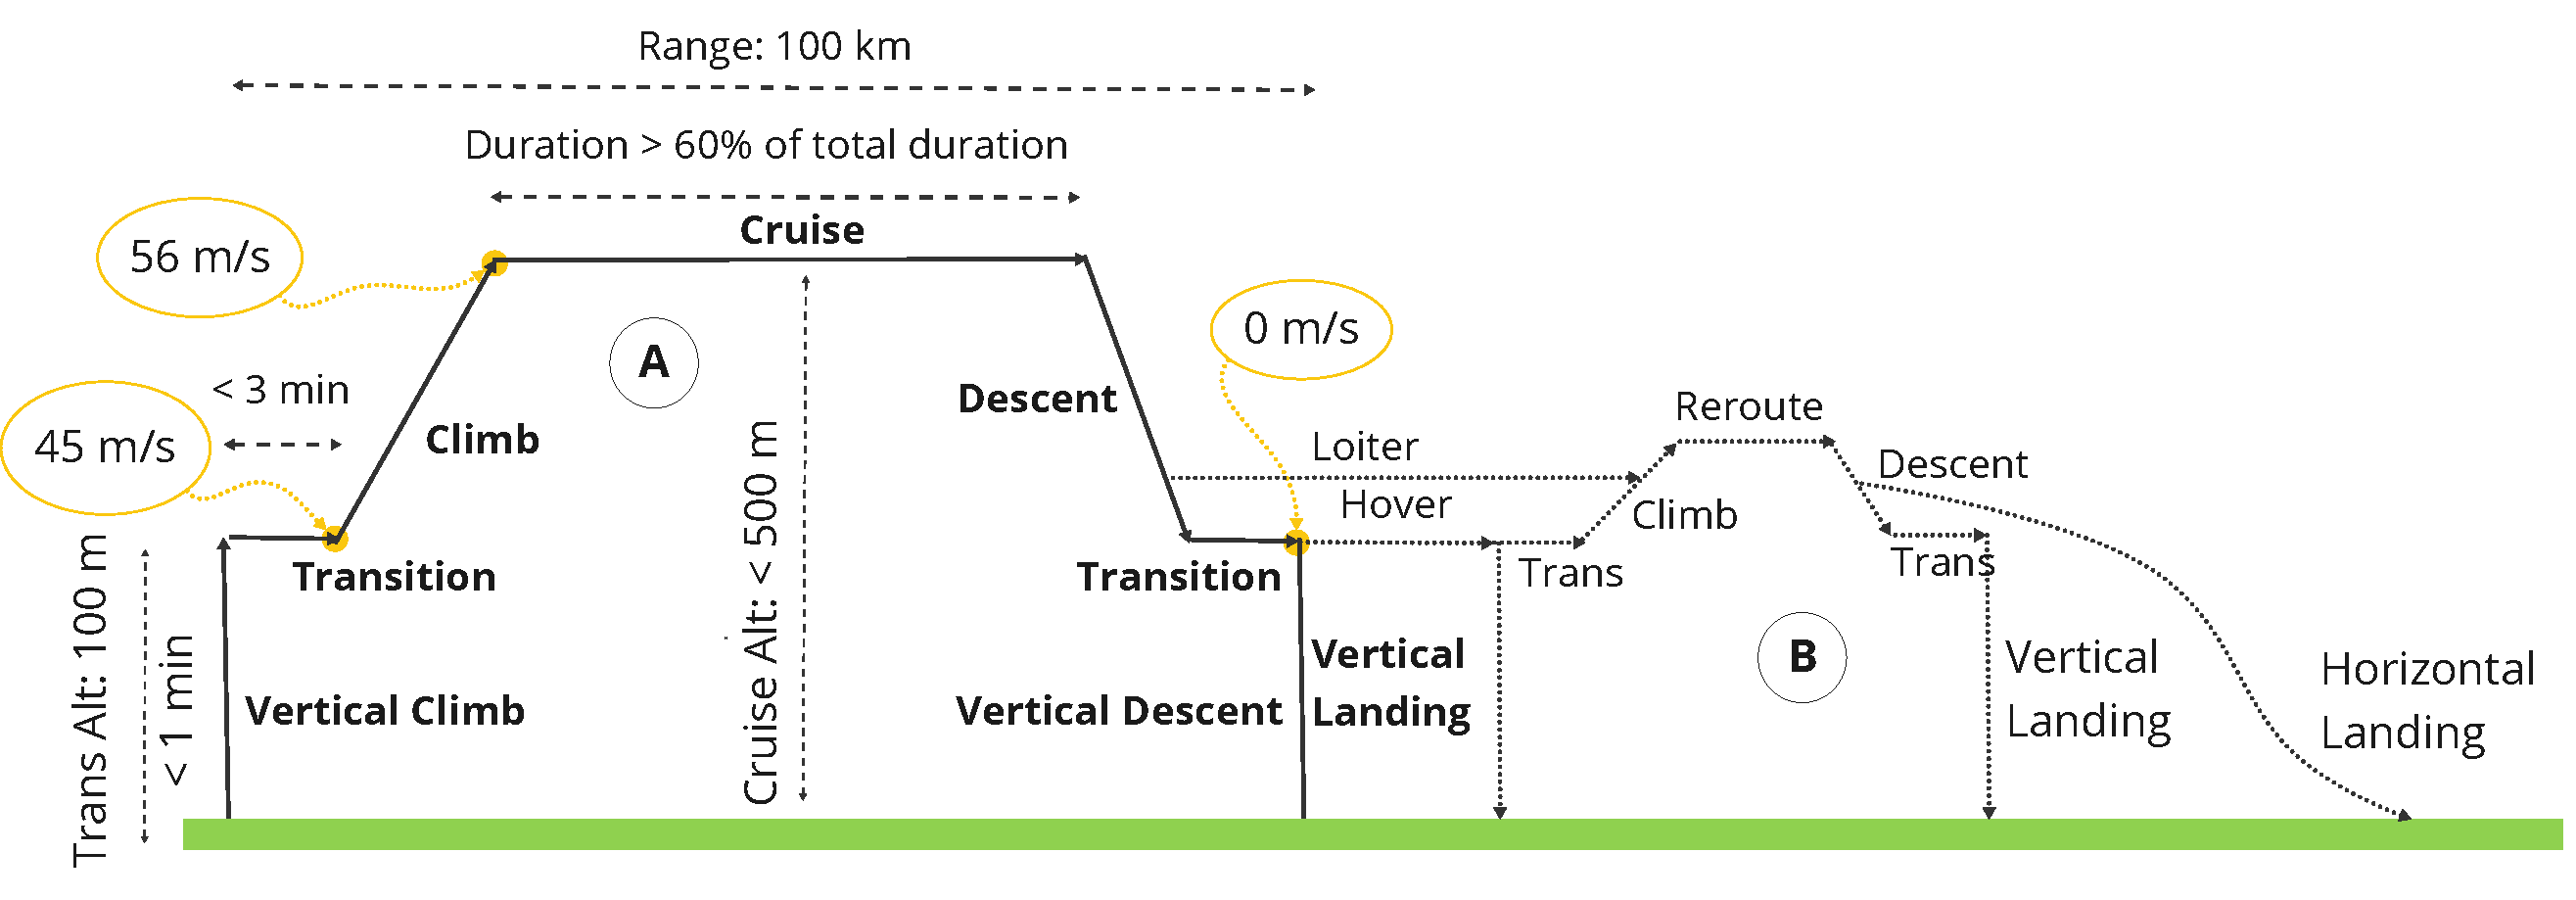
\includegraphics[width=\linewidth]{figures/MissionProfile/Mission_Profile}
    \caption{Mission profile of the eVTOL aircraft}
    \label{fig:mission_profile}
\end{figure}

Considering part A of the profile, the mission starts with a vertical take-off from a vertiport in an urban area.
Then it ascends vertically in the take-off configuration until it has reached transition altitude, set at \qty{100}{\m} above ground level;
this vertical climb phase has a maximum duration of \qty{1}{\minute}.
After reaching the desired altitude, the aircraft transitions to the horizontal configuration.
During the transition, the vehicle accelerates to a velocity of \qty{45}{\m\per\second} while maintaining altitude within a time frame of \qty{3}{\minute}.
Once in the horizontal configuration, the aircraft climbs to the cruise altitude of \qty{500}{\m}.
For cruise, the aircraft will fly at a speed of \qty{200}{\km\per\hour}, for which the minimum duration of the cruise phase is set to be 60\% of the total mission time, for a nominal flight distance of \qty{100}{\km}.
After the cruise, the aircraft descends in horizontal configuration to an altitude of \qty{100}{\m} above ground level and slows down to the transition speed of \qty{45}{\m\per\second}.
While descending, the engine will be throttled back to idle;
then the \textit{Swing} transitions back to the vertical configuration whilst decelerating to a hover.
The aircraft will then descend vertically to the landing site within \qty{1}{\minute} and land.

Part B of \Cref{fig:mission_profile} is illustrated as well since the mission should account for emergency deviations.
The \textit{Swing eVTOL} can use its total battery capacity in an emergency.
Although the battery discharge constraints are set to account for better battery life, there is still enough margin left for an emergency deviation,
paving the way for an emergency diversion to other vertiports.


\section{Mission Optimisation}\label{sec:mission_optimisation}
For the mission profile described in \Cref{sec:mission_overview}, the objective is to minimise the total energy consumption of the aircraft.
To achieve this, a multiphase optimisation approach is used, as described by \citeauthor{traj_opt}~\cite{traj_opt}.
The different mission phases have been modelled and optimised separately.
This enabled utilising different equations of motion, constraints, assumptions, and simplifications for each phase.
The following principles apply to all mission phase optimisations:


\begin{itemize}
    \item The energy consumption per phase is calculated as the sum of the used power multiplied by the time step.
    \item The used power is set as a variable constrained by the maximum engine power.
    \item The power required is calculated using a combination of the equations of motion
    and the power required curve in \Cref{fig:pcurveNOoptimisation}.
\end{itemize}


The different mission phases are optimised, utilising the optimisation software within the Aerosandbox Python package~\cite{aerosandbox}.
This optimisation software utilises the open-source CasADi library~\cite{casadi} for nonlinear optimisation and algorithmic differentiation,
and the IPOPT solver~\cite{IPOPT} for large-scale nonlinear optimisation.

\subsection{Equations of Motion}\label{subsec:equations_of_motion}
The equations of motion for the aircraft are based on Newton's second law of motion.
The aircraft is modelled as a point mass, and the forces acting on it are gravity, thrust, lift, and drag.
The equations of motion are given by:

\begin{align}
    \mathbf{x}(t) &= \int_{t_0}^{t} \mathbf{v} \mathrm{d} t \\
    \mathbf{v}(t) &= \int_{t_0}^{t} \mathbf{a} \mathrm{d} t \\
    \mathbf{a}(t) &= \frac{1}{m} \sum \mathbf{F}(t) \\
    \mathbf{F}(t) &= \mathbf{F}_{\text {gravity }} + \mathbf{F}_{\text {thrust }}(t) + \mathbf{F}_{\text {aero }}(t)
\end{align}
\begin{align}
    \label{eq:simpson}
    \int_{t_{i}}^{t_{i+1}} f(t) dt &\approx \frac{{t_{i+1}}-{t_{i}}}{6}\left[f({t_{i}})+4 f\left(\frac{{t_{i}}+{t_{i+1}}}{2}\right)+f({t_{i+1}})\right] \\
    \int_{t_{0}}^{t_{n}} f(t) dt &\approx \sum_{i=0}^{n-1} \int_{t_{i}}^{t_{i+1}} f(t) dt
\end{align}

Where $\mathbf{x}$ is the position vector, $\mathbf{v}$ is the velocity vector, $\mathbf{a}$ is the acceleration vector, $m$ is the mass of the aircraft, $\mathbf{F}$ is the total force vector acting on the aircraft, $\mathbf{F}_{\text {gravity }}$ is the gravitational force vector, $\mathbf{F}_{\text {thrust }}(t)$ is the thrust force vector produced by the engines, and $\mathbf{F}_{\text {aero }}(t)$ is the aerodynamic force vector consisting of lift and drag.
The equations of motion are integrated using Simpson’s 1/3 rule (\Cref{eq:simpson}),
which is a numerical integration method based on quadratic interpolation.

\subsection{Vertical Climb and Descent Phases}\label{sec:vertical-climb-and-descent-phases}
The vertical climb and descent phases are modelled and optimised using a single point optimisation approach~\cite{traj_opt}.
It begins with the eVTOL resting on the ground and ends when it reaches the transition altitude of \qty{100}{\m} above ground level.
The vertical descent phase begins when the aircraft reaches the transition altitude and ends when it lands on the ground with a maximum vertical speed of \qty{0.5}{\m\per\s}.

\piccaption{Modelled forces acting on the aircraft during the vertical climb and descent phases\label{fig:vertical-fbd}}
\parpic[r][]{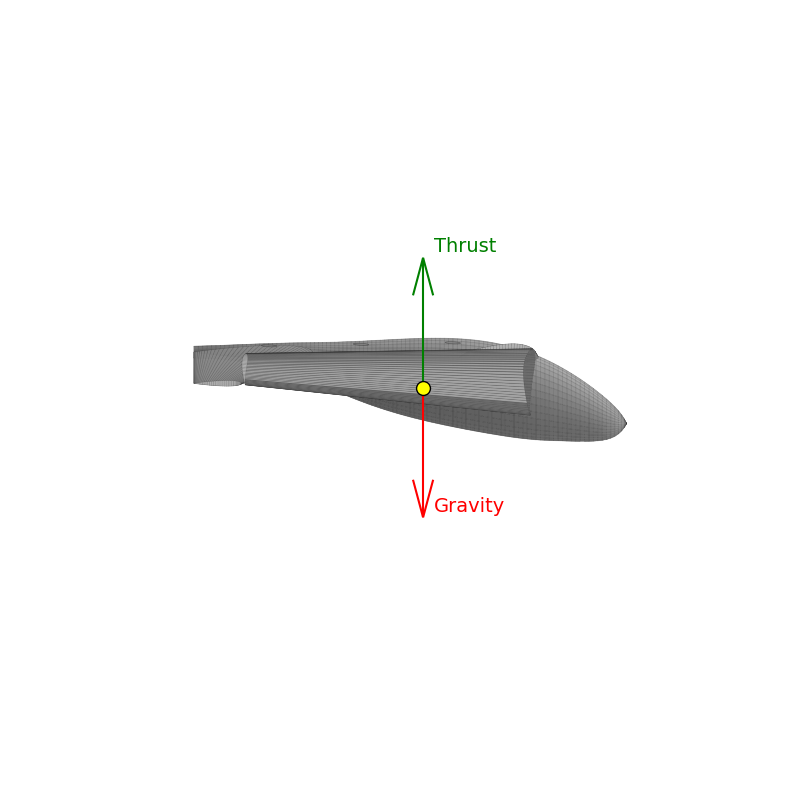
\includegraphics[trim={3.5cm 7cm 3.5cm 6cm},clip,width=0.5\linewidth]{figures/MissionProfile/vertical}}

The optimisation problem is formulated as a point mass model with 1D vertical dynamics.
The aircraft is assumed to be a point mass, and the forces acting on it are gravity and the thrust the engines produce.

Aerodynamic forces are neglected in this phase, as the aircraft is assumed to be in a vertical climb with low vertical speed and no horizontal motion.
To validate this assumption, the worst-case maximum drag force is calculated with the AeroBuildup Aerodynamic engine, as explained in \Cref{sec:AeroBuildup}.
The maximum drag force is found to be \qty{35}{\N},
which is negligible compared to the thrust and weight of the aircraft in the order of \qty{10}{\kN}.

Moreover, the thrust is modelled as a function of the power available and the aircraft’s figure of merit (FM), which measures the rotor system’s efficiency.
The forces acting on the aircraft are visualised in \Cref{fig:vertical-fbd}

The objective of the optimisation is to minimise the aircraft's total energy consumption during the vertical climb phase.
By minimising the total energy instead of the power consumption,
the optimiser makes an efficiency-speed trade-off between climbing in less time and climbing efficiently.
The total energy is calculated as the integral of the power available throughout the climb, which is a decision variable in the optimisation problem, and it is constrained to be less than the maximum engine power.
The optimisation problem also includes constraints on the altitude and vertical speed of the aircraft.
The altitude must increase from zero to the transition altitude, and the vertical speed must be non-positive (indicating upward motion).
The duration of the climb is also a decision variable, and it is constrained to be less than \qty{60}{\s}.
Lastly,
the maximum vertical acceleration and deceleration are constrained to be less than \qty{2}{\m\per\s\squared} to ensure
a smooth ride for the passengers.
The solution to the optimisation problem provides the optimal thrust level as a function of time and altitude,
which minimises the total energy consumption of the aircraft during the vertical climb phase.

\begin{figure}[!hptb]
    \centering
    \begin{subfigure}[b]{0.45\textwidth}
        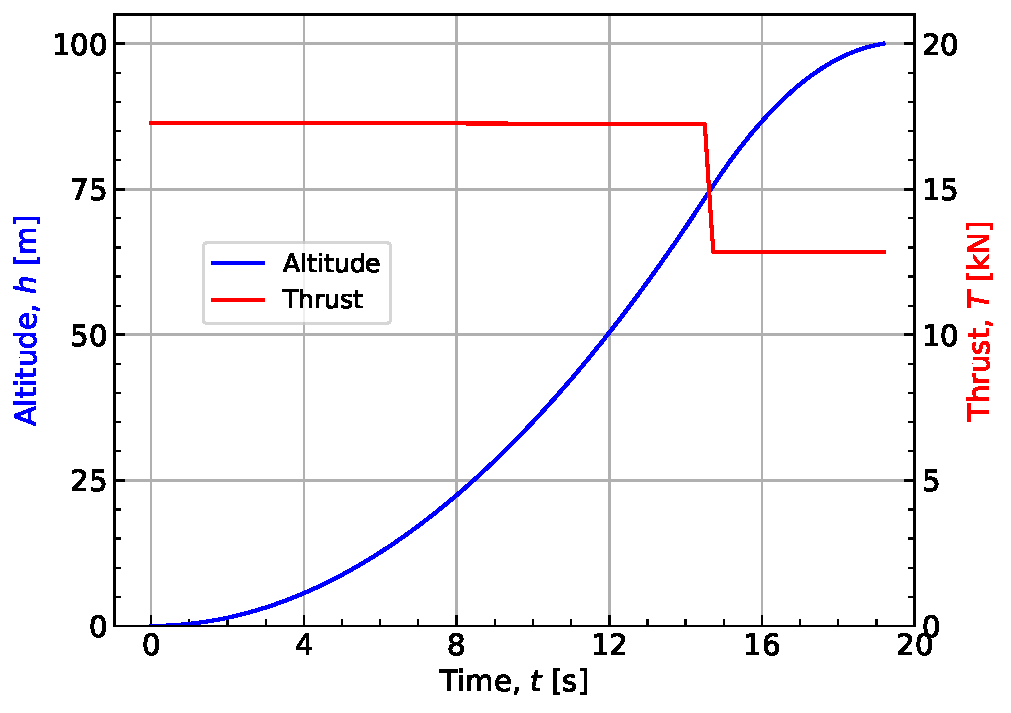
\includegraphics[width=\textwidth]{figures/MissionProfile/VerticalClimb_over_time}
        \caption{Altitude and total thrust over time of the vertical climb phase}
        \label{fig:vertical_climb_over_time}
    \end{subfigure}
    \hfill
    \begin{subfigure}[b]{0.45\textwidth}
        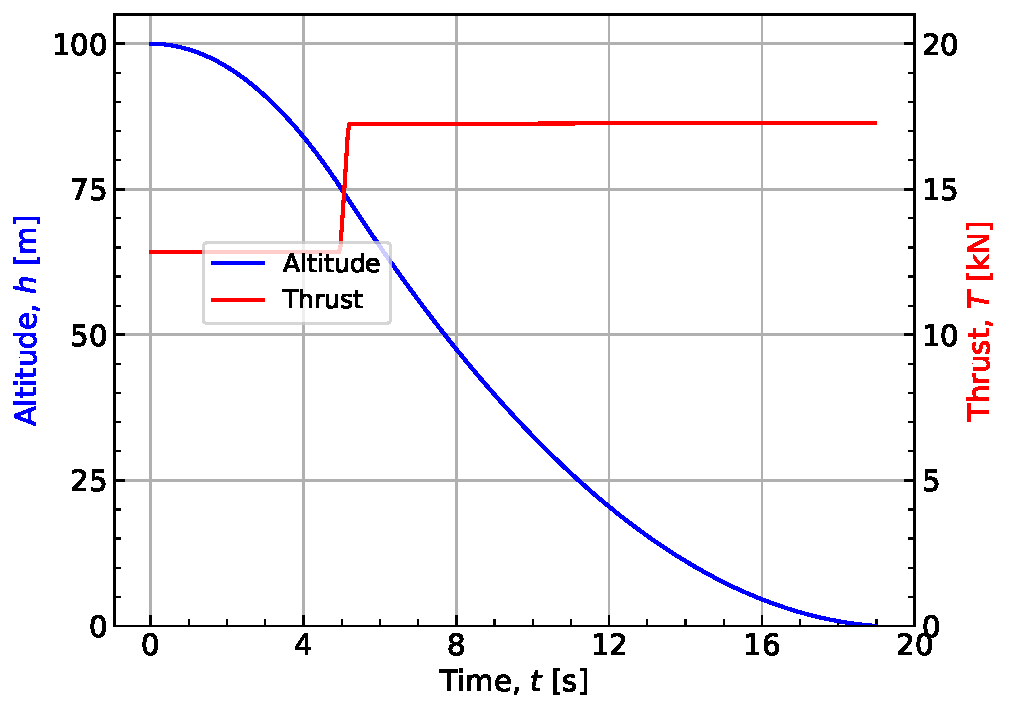
\includegraphics[width=\textwidth]{figures/MissionProfile/VerticalDescent_over_time}
        \caption{Altitude and total thrust over time of the vertical descent phase}
        \label{fig:vertical_descent_over_time}
    \end{subfigure}
    \caption{Altitude and total thrust over time of the vertical climb and descent phases}
    \label{fig:vertical_climb_descent_over_time}
\end{figure}

As can be seen in \Cref{fig:vertical_climb_descent_over_time},
the vertical climb and descent phases are completed within \qty{20}{\s}, well within the maximum duration of \qty{60}{\s}.
The total energy consumption of the aircraft during both phases is roughly \qty{1.6}{\kWh}.

\subsection{Transition Phase}\label{subsec:transition}
The transition phase is when the aircraft changes from vertical to horizontal flight configuration.
This phase is modelled and optimised using a single point optimisation approach~\cite{traj_opt}, similar to the vertical climb phase.
The optimisation problem is formulated as a point mass model with 1D horizontal dynamics.
Where the power required is calculated at each point during the transition and over the velocity range.
This required power consists of induced, profile, and parasite power, which is explained in more detail in \Cref{fig:pcurveNOoptimisation}.
Furthermore, the additional thrust needed to accelerate the aircraft is a free variable in the optimisation problem.
The power used for acceleration is computed from this additional thrust,
taking into account the direction the engines are pointing at the current transition parameter, as can be seen in \Cref{fig:transition-opt-fbd}.

\piccaption{Modelled forces acting on the aircraft during the transition phase\label{fig:transition-opt-fbd}}
\parpic[r][]{
\includegraphics[trim={5cm 6cm 3.5cm 5cm},clip,width=0.5\linewidth]{figures/MissionProfile/trans}}

As can be noted from the figure, the extra thrust is split into a vertical and horizontal component.
The extra vertical thrust is then ignored, as the required vertical speed is to be zero to simplify the model.
Therefore, the aircraft will gain altitude during the transition phase in a real-world scenario.
This would make the following climb phase more efficient, as the aircraft would start at a higher altitude.

The second free variable in the optimisation problem is the transition parameter used to determine the aircraft’s configuration between vertical and horizontal flight.
The transition parameter is constrained to start at one (vertical flight) and end at zero (horizontal flight).
The transition parameter is also constrained to be a smooth decreasing function of time to ensure a smooth transition between the two configurations.
It should be noted that the power required curve is a function of the transition parameter, as the aircraft’s configuration affects the aerodynamic forces acting on it.
Those aerodynamic forces are computed using the AeroBuildup Aerodynamic engine, as explained in \Cref{sec:AeroBuildup}.

The horizontal speed is required to increase from zero to the transition speed, and the transition duration is constrained to be less than \qty{180}{\s}.
The eventual solution to the optimisation problem provides the optimal power available, power required, thrust level, velocity, and control inputs as functions of time, distance, and velocity, which minimises the maximum power required during the transition phase.
The control inputs include the angle of attack and the transition parameter, which determines the aircraft’s configuration between vertical and horizontal flight.

\begin{figure}[!hptb]
    \centering
    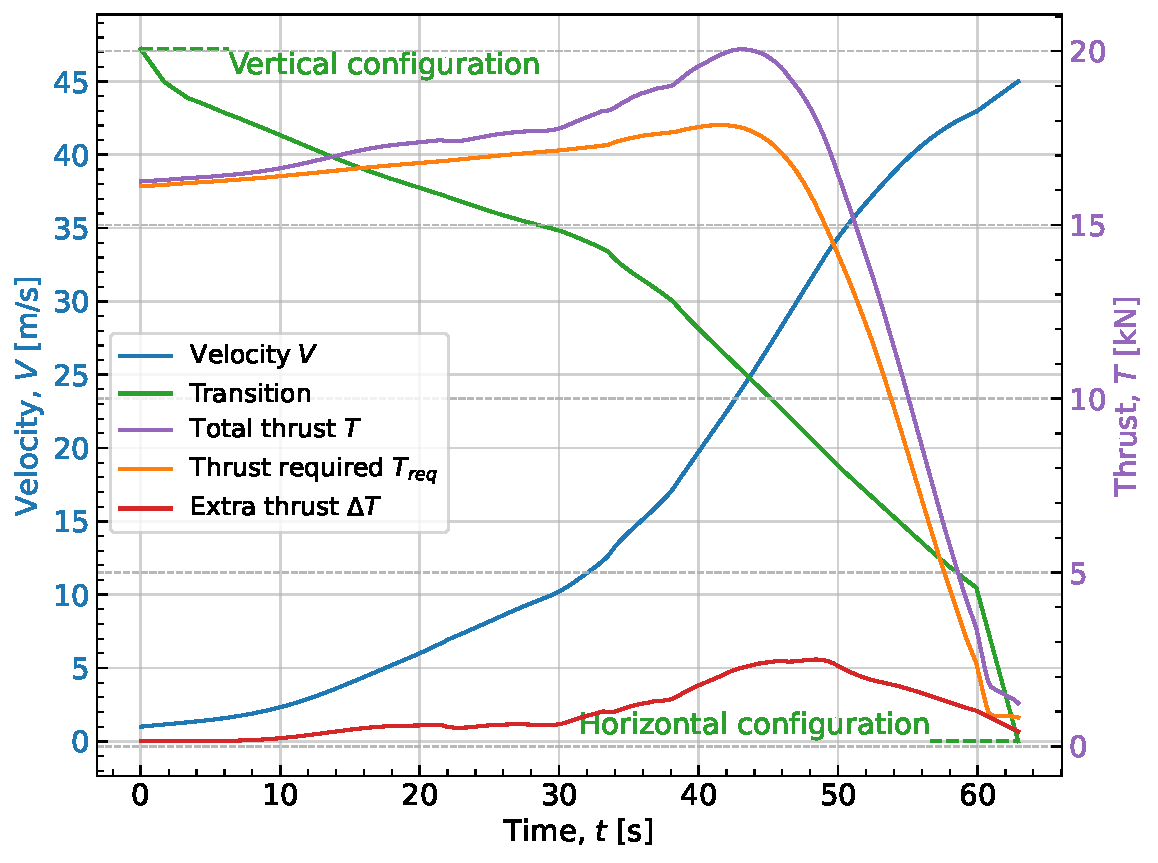
\includegraphics[width=0.85\linewidth]{figures/MissionProfile/transition_free_variables}
    \caption{Extra horizontal thrust, transition parameter, and velocity over time during the transition phase}
    \label{fig:transition-opt-vars}
\end{figure}

\begin{figure}[!hptb]
    \centering
    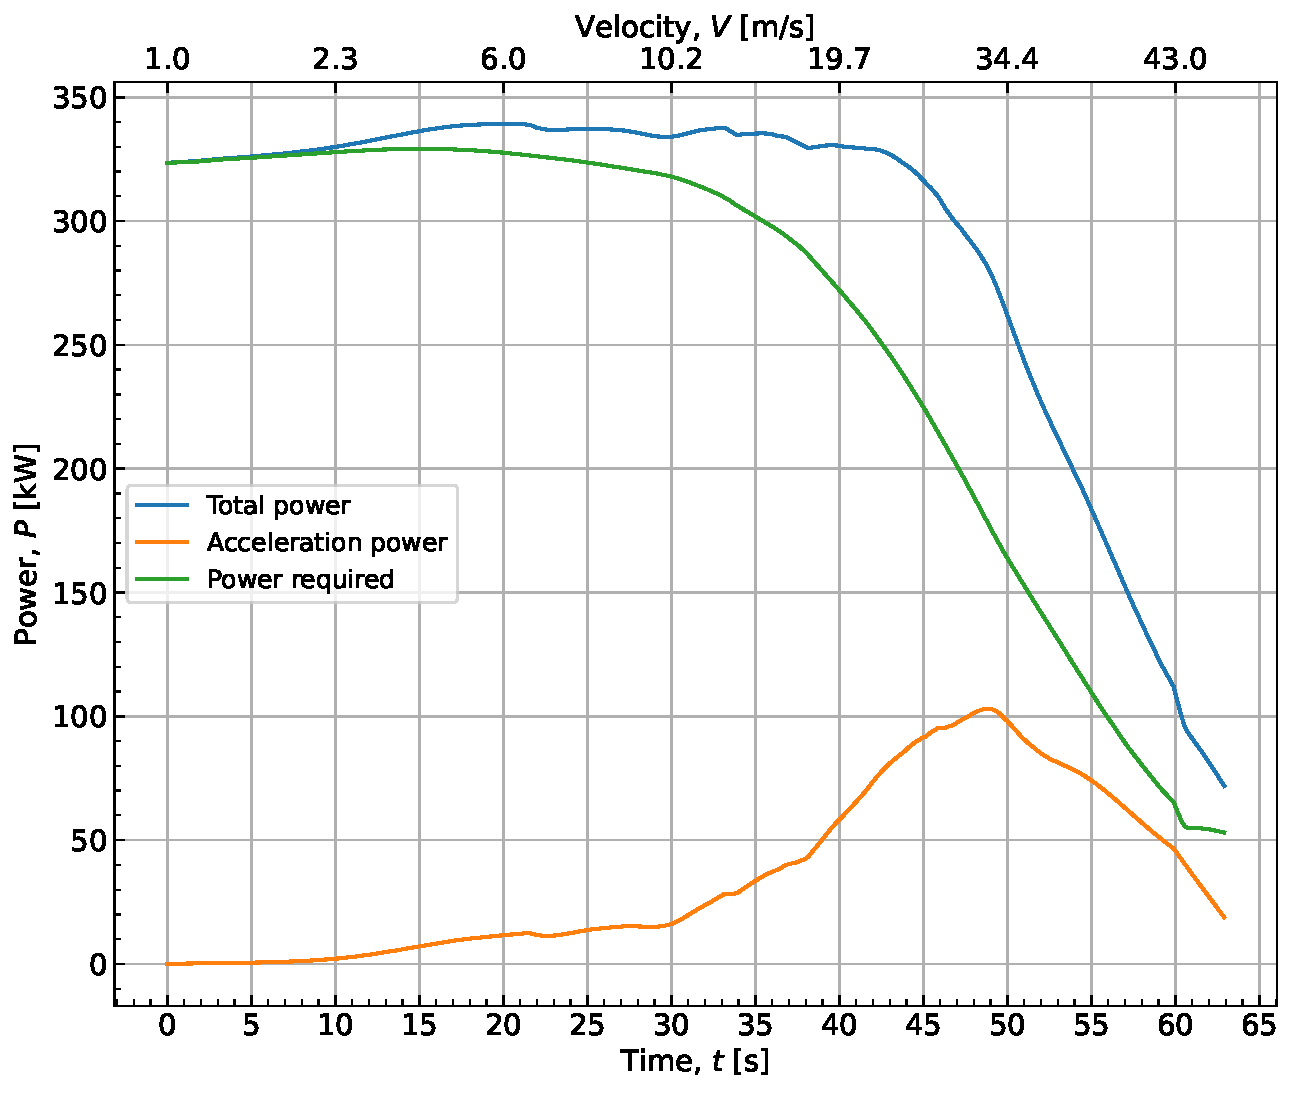
\includegraphics[width=0.85\linewidth]{figures/MissionProfile/power_over_velocity_and_time}
    \caption{Power required and acceleration power over velocity and time during the transition phase.
    A detailed explanation of the power required curve is given in \Cref{sec:missionpowercurve}}
    \label{fig:transition_power_over_velocity_and_time}
\end{figure}

As can be seen in \Cref{fig:transition-opt-vars}, the transition phase starts with the aircraft in vertical flight configuration,
with a horizontal speed of \qty{1}{\m\per\s} to avoid division by zero in the power required curve.
The aircraft then slowly transitions, increasing the forward momentum.
As the vehicle transitions, the required thrust increases to maintain the desired altitude (see \Cref{fig:transition-opt-fbd}).
When the aircraft flies with a horizontal velocity of around \qty{10}{\m\per\s} after \qty{30}{\s} in the transition phase,
the required power starts to decrease, as seen in \Cref{fig:transition_power_over_velocity_and_time}.
From this point, the aircraft starts to accelerate and transition more aggressively, keeping the maximum power peak as low as possible.
The remaining $\Delta V$ of around \qty{35}{\m\per\s}, and 70\% of the transition, is achieved in the second half of the transition phase.
The transition phase ends with the aircraft flying with a velocity of \qty{45}{\m\per\s} in horizontal flight configuration.
The transition phase is completed in \qty{63}{\s}, which is well within the maximum duration of \qty{180}{\s}.

The second transition phase, however, has not been modelled, as it is assumed to be less power-intensive than the first.
The aircraft will not require additional thrust to decelerate to the hover velocity of \qty{0}{\m\per\s}.
Thus, for the total mission, the power is assumed to increase linearly from cruise power to hover power.

\subsection{Climb, Cruise, and Descent Phases}\label{subsec:climb_cruise_descent}
The climb, cruise, and descent phases are modelled and optimised using a single-phase full-dynamics optimisation approach~\cite{traj_opt}.
The optimisation problem is formulated as a point mass model with 2D dynamics, where the aircraft is assumed to be a point mass, and the forces acting on it are gravity, the thrust produced by the engines, and the aerodynamic forces.
The thrust is the free variable in the optimisation problem.
Moreover, the general 2D equations of motion are used to calculate the aircraft’s velocity, acceleration, and position at each point during the climb, cruise, and descent phases.
The forces acting on the aircraft are visualised in \Cref{fig:horizontal-fbd}

\piccaption{Modelled forces acting on the aircraft during the climb, cruise, and descent phases\label{fig:horizontal-fbd}}
\parpic[r][]{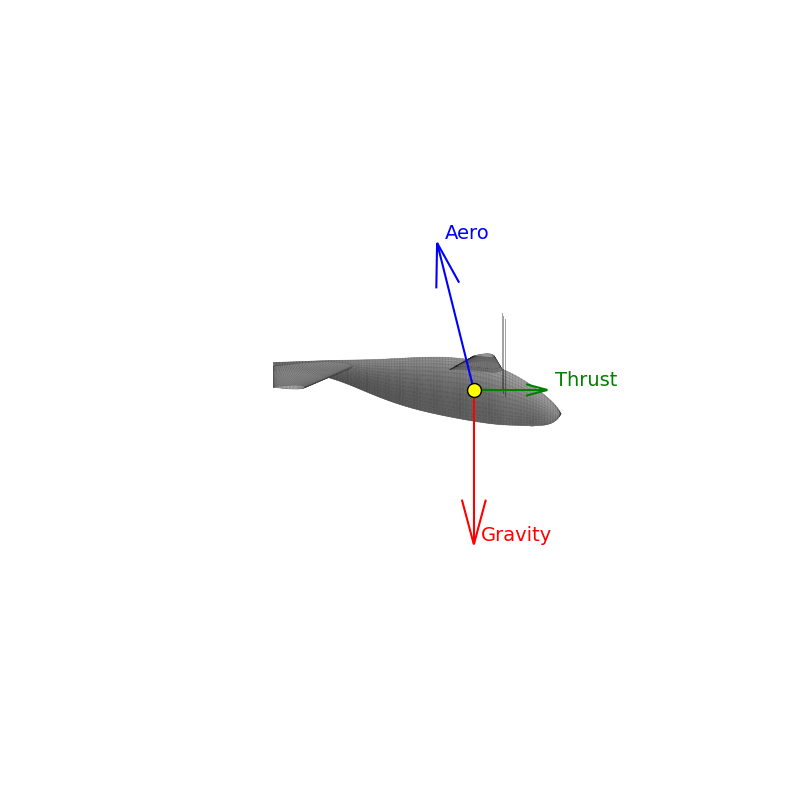
\includegraphics[trim={6cm 6cm 3.5cm 5cm},clip,width=0.5\linewidth]{figures/MissionProfile/horizontal}}

The objective of the optimisation is to minimise the total energy consumption of the aircraft during these phases.
The total energy is calculated as the integral of the power available over the duration of each phase, which is calculated as a function of the thrust produced by the engines and the aircraft’s velocity,
based on the power curve in \Cref{fig:pcurveNOoptimisation}.

The optimisation problem includes constraints on the aircraft's altitude, vertical speed, and horizontal speed.
The altitude is required to increase from the transition altitude to the cruise altitude during the climb phase, remain constant at the cruise altitude during the cruise phase, and decrease from the cruise altitude to the transition altitude during the descent phase.
The vertical speed is required to be positive (indicating upward motion) during the climb phase, zero (indicating no vertical motion) during the cruise phase, and negative (indicating downward motion) during the descent phase.
The horizontal speed is required to increase from the transition speed to the cruise speed during the climb phase, remain constant at the cruise speed during the cruise phase, and decrease from the cruise speed to the transition speed during the descent phase.
The duration of each phase is also a free variable, and it is constrained to be less than the maximum duration of the phase.
The solution to the optimisation problem provides the optimal power available, thrust level, and alpha as functions of time, which minimise the total energy consumption of the aircraft during the climb, cruise, and descent phases.

\begin{figure}[!hptb]
    \centering
    
\includegraphics[width=0.9\linewidth]{figures/MissionProfile/alt_hor_ver_vel_power_over_distance}
    \caption{Altitude, horizontal speed, vertical speed, and engine power over distance during the climb, cruise, and descent phases}
    \label{fig:climb_cruise_descent_over_distance}
\end{figure}

As can be seen in \Cref{fig:climb_cruise_descent_over_distance}, the climb phase starts with the aircraft at the transition altitude of \qty{100}{\m} above ground level.
The aircraft then climbs to the cruise altitude of \qty{500}{\m} above ground level,
with an average vertical speed of \qty{1.5}{\m\per\s} and an average power of \qty{80}{\kW}.
The fluctuation in the vertical speed is likely due to anomalies from the optimisation,
but it is not expected to influence the results significantly.
The cruise phase starts with the aircraft at the cruise altitude of \qty{500}{\m} above ground level,
and the aircraft flies at a constant horizontal speed of \qty{200}{\km\per\hour},
with an average power level of \qty{50}{\kW}.
The descent phase starts with the aircraft at the cruise altitude of \qty{500}{\m} above ground level,
and the aircraft descends to the transition altitude of \qty{100}{\m} above ground level,
with an average vertical speed of \qty{-2.4}{\m\per\s}, and average idling power of \qty{0.1}{\kW}.
The descent phase ends with the aircraft at the transition altitude of \qty{100}{\m} above ground level.


\section{Flight Performance}\label{sec:flight_performance}
The flight performance of the \textit{Swing eVTOL} is evaluated based on the optimised mission profile described in \Cref{sec:mission_optimisation}.
The performance metrics include the total energy consumption, the maximum power required, the maximum thrust level, and the flight time for each phase of the mission.
The performance metrics are calculated for the nominal mission profile and different mission profiles with variations in the mission parameters, such as increased range.
In the future, other mission profiles can be evaluated as well,
such as increased cruise velocity or different payload configurations.

\subsection{Nominal Mission Profile Results}\label{sec:nominal_mission_profile_results}
The optimised mission profile for the \textit{Swing} is shown in \Cref{fig:nominal_mission_profile_results}, including altitude and engine power over distance and time.
The energy distribution over the different phases of the mission is shown in \Cref{fig:nominal_energy_distribution}.
Where the total energy consumption of the aircraft during the nominal mission profile is \qty{34}{\kWh}.
The maximum power required by the aircraft during the mission is \qty{343}{\kW},
and the maximum thrust level is \qty{20.2}{\kN}.
Furthermore, the total flight time of the nominal mission profile is \qty{32}{\minute}.
The results show that the aircraft can complete the mission with the given constraints while minimising the total energy consumption and the maximum power required.

\subsection{Mission Profile with Maximum Range}\label{sec:mission_profile_max_range}
The mission profile for the maximum range is found by increasing the total distance to \qty{250}{\km}.
Extending the cruise period for the maximum amount of time whilst keeping the State of Charge of the battery between 90\% and 20\%, which is explained in greater detail in \Cref{ch:eps}
Assuming that only the Climb, Cruise, and Descent phases are affected by the increased range,
only the horizontal optimisation of \Cref{subsec:climb_cruise_descent} is rerun.
The optimisation results are shown in \Cref{fig:climb_cruise_descent_over_distance_max_range}.
As can be seen in the figure, it is more efficient to fly at a higher altitude during the cruise phase,
as the power required is lower at higher altitudes.

\begin{figure}[!hptb]
    \centering
    
\includegraphics[width=0.9\linewidth]{figures/MissionProfile/alt_hor_ver_vel_power_over_distance_max_range}
    \caption{Altitude, horizontal speed, vertical speed,
        and engine power over distance during the climb, cruise, and descent phases for the maximum range mission profile}
    \label{fig:climb_cruise_descent_over_distance_max_range}
\end{figure}


The new mission profile for the maximum range is shown in \Cref{fig:max_range_mission_results}, and the energy distribution over the different phases of the mission is shown in \Cref{fig:energy_distribution_max_range}.
It can be seen that the climb phase is now the most energy-intensive phase of the mission since the aircraft has to climb to a higher altitude.
The energy for the cruise phase went down relative to the total mission energy,
as the aircraft spends more time in the climb and descent phases.
The total energy consumption of the aircraft during the mission with maximum range is \qty{70}{\kWh}.
Subsequently, the total flight time of the mission with maximum range concludes \qty{79}{\minute}.

\begin{figure}[!hptb]
\centering
\begin{subfigure}[b]{0.8\textwidth}
    \centering
    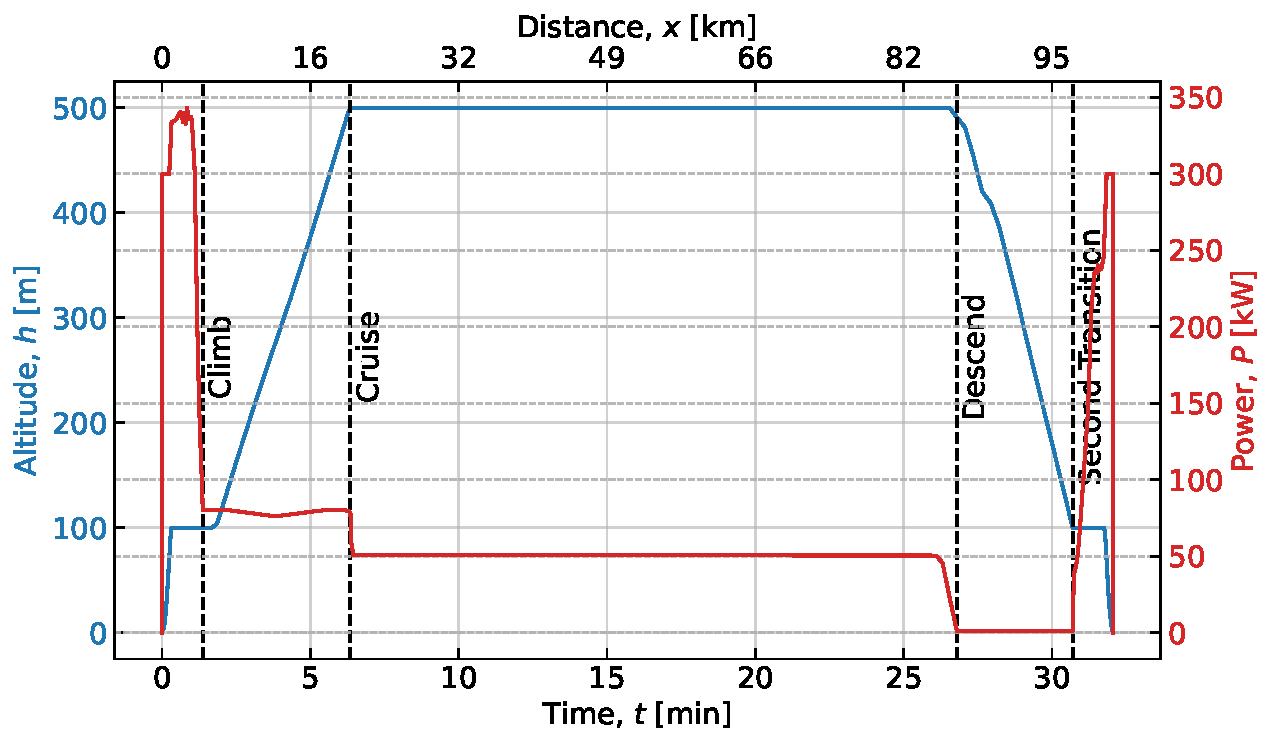
\includegraphics[width=.95\textwidth]{figures/MissionProfile/mission_profile_over_time_and_distance}
    \caption{Altitude and engine power over distance and time of the nominal mission profile}
    \label{fig:nominal_mission_profile_results}
\end{subfigure}
~
\begin{subfigure}[b]{0.8\textwidth}
    \centering
    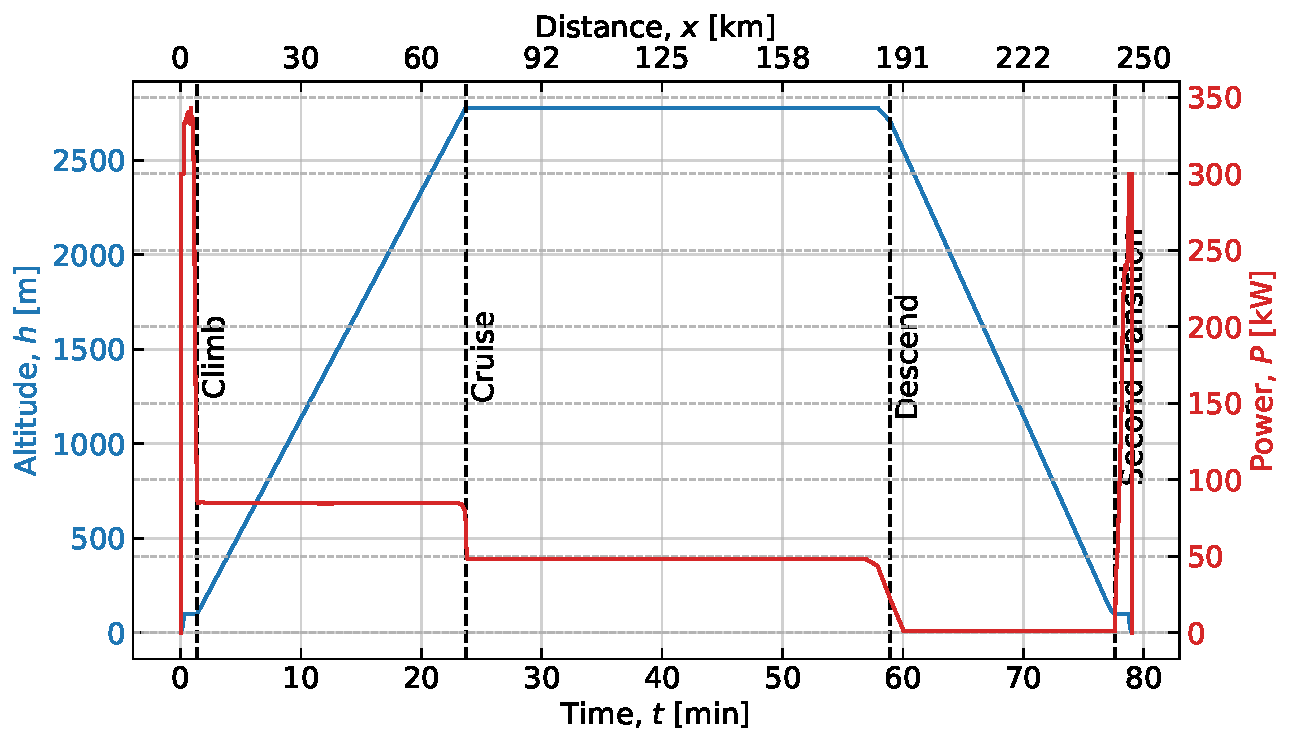
\includegraphics[width=0.95\textwidth]{figures/MissionProfile/mission_profile_over_time_and_distance_max_range}
    \caption{Altitude and engine power over distance and time of the mission profile with maximum range}
    \label{fig:max_range_mission_results}
\end{subfigure}
\caption{Mission profile results for the nominal mission profile and the mission profile with maximum range}
\label{fig:mission_profile_results}
\end{figure}


\begin{figure}[!hptb]
    \begin{subfigure}[b]{0.49\textwidth}
        \centering
        
\includegraphics[width=0.95\linewidth]{figures/MissionProfile/energy_distribution}
        \caption{Energy distribution of the nominal mission profile}
        \label{fig:nominal_energy_distribution}
    \end{subfigure}
    \hfill
    \begin{subfigure}[b]{0.49\textwidth}
        \centering
        
\includegraphics[width=0.95\linewidth]{figures/MissionProfile/energy_distribution_max_range}
        \caption{Energy distribution of the mission profile with maximum range}
        \label{fig:energy_distribution_max_range}
    \end{subfigure}
    \caption{Energy distribution over the different phases of the mission profiles}
    \label{fig:energy_distribution}
\end{figure}
